\documentclass{article}

\usepackage{../swiftnav}
\usepackage{../swiftnav_tikz}

\rhead{Swift Navigation NAP}

\usepackage{draftwatermark}
\SetWatermarkLightness{0.85}
\SetWatermarkText{Preliminary}
\SetWatermarkScale{4}

\usetikzlibrary{calc,fit,matrix,chains}

\usetikzlibrary{shapes.geometric,shapes.arrows,decorations.pathmorphing}
\usetikzlibrary{scopes,positioning,arrows}

\version{2.2.0}
\title{Swift Navigation NAP\\(Navigation/Acquisition Processor)}
\author{Swift Navigation}
\date{\today}

\begin{document}

\maketitle

\raggedcolumns
\begin{multicols}{2}

\section*{Overview}

The Swift Navigation NAP (Navigation/Acquisition Processor) is a multi-function 
hardware accelerator, implemented using a Xilinx Spartan 6 FPGA, for the lowest levels 
of signal processing in the Swift Navigation GNSS Receiver. It groups correlators into 
channels with specific purposes while allowing the user a large amount of control and 
flexibility.

The Swift NAP includes 12?? tracking channels with lower level interfaces, each containing 
6 correlators : one each for early I, early Q, prompt I, prompt Q, late i, and late q (half 
chip??variable spacing). It includes one serial search acquisition channel that searches 15?? 
code phases in parallel (half chip spacing), at 81.84?? MHz (5x sample clock), which gives 
an acquisition speed 75x?? that of real time. In addition, it includes a spectrum power 
analyzation channel for detecting continuous wave interference, and a 5?? tap IIR filter for 
continuous-wave rejection between the frontend samples and the acquisition and tracking channels.
\columnbreak

\section*{Features}
\begin{itemize}
  \bulletnoindent
  \item 3 bit samples
  \item 16.368MHz sample clock frequency
  \item 12?? tracking channels
  \item 1/75?? real time serial search acquisition
  \item Dedicated CW (continuous-wave) detection channel
  \item IIR filter for CW filtering
  \item Low level control
\end{itemize}

\pagebreak
\tableofcontents
\pagebreak

\end{multicols}

\section{Block Diagram}
\begin{center}
  \begin{tikzpicture}[point/.style={circle,inner sep=0pt,minimum size=2pt,fill=red},
                      tip/.style={->,shorten >=1pt}]

    \tikzstyle{antenna} = [draw,isosceles triangle,minimum width=5mm,shape border rotate=300,color=red]
    \tikzstyle{block} = [draw, fill=orange!20, rectangle, text width=1.5cm, minimum height=1.8cm, minimum width=1.8cm, line width=0.5pt]
    \def\filterSS{\node[block]{};\draw[line width=1pt] (-4mm,-2mm) to[in=220,out=40] (4mm,-2mm) 
                                                        (-4mm,0mm) to[in=220,out=40] (4mm,0mm) 
                                                        (-4mm,2mm) to[in=220,out=40] (4mm,2mm)
                                                       (-1mm,-1mm) to (1mm,1mm);}
    \tikzstyle{connection_matrix} = [matrix of nodes,
          column sep=0.45cm,
          row sep=0.45cm,
          anchor=center,
          nodes={anchor=center}] 

    \tikzstyle{blocks_matrix} = [matrix of nodes,
          column sep=0.25cm,
          row sep=0.25cm,
          anchor=center,
          nodes={anchor=center}] 
    
    %Draw blocks
    \matrix[blocks_matrix] (blocks) at (0,0) {
       %First row
       \node[below] (from frontend) {From Frontend}; & \node[minimum width=1.0cm] {}; & & \filterSS & & \\
       %Second row
       & & \node[block] (cw) {CW \ \ \ Detection Correlator}; & & \node[block] (acq) {Acquisition Correlator}; & \node[block] (trackfront) {Tracking Correlators}; & \node[minimum width=2cm] {}; & \\
       %Third row
       & & \node[] (cw nodes center) {}; & \node[] (filter nodes center) {}; & \node[] (acq nodes center) {}; & \node[] (track nodes center) {}; & \node[] (nap stm arrows center) {}; & \node[minimum height=3cm] (to stm center) {}; \\
    };
    %"To STM" label
    \node[right of=to stm center] {To STM};
    %Assign filter to blocks-1-4
    \coordinate (filter_west) at (blocks-1-4.west);
    \coordinate (filter_east) at (blocks-1-4.east);
    \coordinate (filter_south) at (blocks-1-4.south);
    \coordinate (filter_north) at (blocks-1-4.north);

    %CW signal connections
    \matrix[connection_matrix] (cw nodes south) at (cw.south) {
      |[coordinate]| & |[coordinate]| & |[coordinate]| & |[coordinate]| \\};
    \matrix[connection_matrix] (cw nodes below) at (cw nodes center) {
       & |[coordinate]| & & & & |[coordinate]| \\
       & & & & |[coordinate]| & \\
       & & & |[coordinate]| & & \\
       & & |[coordinate]| & & & \\
       & |[coordinate]| & & & & \\
       |[coordinate]| & & & & & \\};

    %Filter signal connections
    \matrix[connection_matrix] (filter nodes south) at (filter_south) {
      |[coordinate]| & |[coordinate]| & |[coordinate]| & |[coordinate]| \\};
    \matrix[connection_matrix] (filter nodes below) at (filter nodes center) {
       & |[coordinate]| & & & & |[coordinate]| \\
       & & & & |[coordinate]| & \\
       & & & |[coordinate]| & & \\
       & & |[coordinate]| & & & \\
       & |[coordinate]| & & & & \\
       |[coordinate]| & & & & & \\};

    %Acq signal connections
    \matrix[connection_matrix] (acq nodes south) at (acq.south) {
      |[coordinate]| & |[coordinate]| & |[coordinate]| & |[coordinate]| \\};
    \matrix[connection_matrix] (acq nodes below) at (acq nodes center) {
       & |[coordinate]| & & & & |[coordinate]| \\
       & & & & |[coordinate]| & \\
       & & & |[coordinate]| & & \\
       & & |[coordinate]| & & & \\
       & |[coordinate]| & & & & \\
       |[coordinate]| & & & & & \\};

    %Tracking signal connections
    \matrix[connection_matrix] (track nodes south) at (trackfront.south) {
      |[coordinate]| & |[coordinate]| & |[coordinate]| & |[coordinate]| \\};
    \matrix[connection_matrix] (track nodes below) at (track nodes center) {
       & & & & & |[coordinate]| \\
       & & & & |[coordinate]| & \\
       & & & |[coordinate]| & & \\
       & & |[coordinate]| & & & \\
       & |[coordinate]| & & & & \\
       |[coordinate]| & & & & & \\};

    %STM signal connections
    \matrix[connection_matrix] (nap nodes) at (nap stm arrows center) {
      |[coordinate]| \\ |[coordinate]| \\ |[coordinate]| \\ |[coordinate]| \\};
    \matrix[connection_matrix] (stm nodes) at (to stm center) {
      |[coordinate]| \\ |[coordinate]| \\ |[coordinate]| \\ |[coordinate]| \\};

    %Label for filter
    \draw (filter_north) node[above, name=filter label, inner sep=1mm] {IIR Filter};

    %Other tracking channel boxes, then redraw original
    \draw let \p1=(trackfront) in ($(\x1+3mm, \y1+3mm)$) node[block,text width=1.7cm] (trackback) {};
    \draw let \p1=(trackfront) in ($(\x1+1.5mm, \y1+1.5mm)$) node[block,text width=1.7cm] (trackmid) {};
    \draw (trackfront) node[block,text width=1.7cm] (trackfront) {Tracking Correlators};

    %Frontend clock initial segment and frontend data connections
    \path let \p0=(from frontend),\p1=(filter_west) in 
       coordinate(clock sig first seg orig) at ($(\x0,\y1) + (15mm,-6mm)$)
       coordinate(clock sig first seg dest) at ($(\x0,\y1) + (20mm,-6mm)$)
       coordinate(frontend data orig) at ($(\x0,\y1) + (15mm,0mm)$);
    \draw[>-,color=black!100,thick] (clock sig first seg orig) -- node[right,very near end,font=\scriptsize,text width=1cm] {Frontend\\Clock} (clock sig first seg dest);
    \draw[-,color=black!100,thick] (clock sig first seg dest) |- node[name=clock sig downward] {} (cw nodes below-5-2);
    \draw[>->,thick] (frontend data orig) -| node[above,font=\scriptsize] {3 bit samples} (cw);
    \path let \p0=(frontend data orig),\p1=(cw) in coordinate (filter data sig orig) at ($(\x1,\y0)$);
    \draw[->,thick] (filter data sig orig) -- (filter_west);

    %Data signal connections
    \draw[->,thick] (filter_east) -| (acq);
    \path let \p0=(filter_east),\p1=(acq),\p2=(trackmid),\p3=(trackback.north) in 
      coordinate (track data sig orig) at ($(\x1,\y0)$)
      coordinate (track data sig dest) at ($(\x2,\y3)$);
    \draw[->,thick] (track data sig orig) -| node[above,near start,font=\scriptsize] {1 bit filtered} (track data sig dest);

    %Clock signal multipliers
    \node[block] (cw multiplier) at (cw nodes below-1-2) [minimum width=5mm,minimum height=5mm,text width=3mm] {x3};
    \node[block] (filter multiplier) at (filter nodes below-1-2) [minimum width=5mm,minimum height=5mm,text width=3mm] {x4};
    \node[block] (acq multiplier) at (acq nodes below-1-2) [minimum width=5mm,minimum height=5mm,text width=3mm] {x5};

    %Interrupt line connections
    \draw[<-,color=orange!100,thick] (cw nodes below-4-3) -- (cw nodes south-1-2);
    \draw[<-,color=orange!100,thick] (filter nodes below-4-3) -- (filter nodes south-1-2);
    \draw[<-,color=orange!100,thick] (acq nodes below-4-3) -- (acq nodes south-1-2);
    \draw[<-,color=orange!100,thick] (track nodes below-4-3) -- (track nodes south-1-2);
    \draw[-,color=orange!100,thick] (cw nodes below-4-3) -- (nap nodes-3-1);
    \draw[>->,color=orange!100,thick] (nap nodes-3-1) -- node[above,font=\scriptsize,color=black] {IRQ} (stm nodes-3-1);
    %Timing strobe line connections
    \draw[->,color=blue!100,thick] (cw nodes below-3-4) -- (cw nodes south-1-3);
    \draw[->,color=blue!100,thick] (filter nodes below-3-4) -- (filter nodes south-1-3);
    \draw[->,color=blue!100,thick] (acq nodes below-3-4) -- (acq nodes south-1-3);
    \draw[->,color=blue!100,thick] (track nodes below-3-4) -- (track nodes south-1-3);
    \draw[-,color=blue!100,thick] (cw nodes below-3-4) -- (nap nodes-2-1);
    \draw[<-<,color=blue!100,thick] (nap nodes-2-1) -- node[above,font=\scriptsize,color=black] {Timing Strobe} (stm nodes-2-1);
    %SPI 
    \draw[<->,color=red!100,thick] (cw nodes below-2-5) -- (cw nodes south-1-4);
    \draw[<->,color=red!100,thick] (filter nodes below-2-5) -- (filter nodes south-1-4);
    \draw[<->,color=red!100,thick] (acq nodes below-2-5) -- (acq nodes south-1-4);
    \draw[<->,color=red!100,thick] (track nodes below-2-5) -- (track nodes south-1-4);
    \draw[-,color=red!100,thick] (cw nodes below-2-5) -- (nap nodes-1-1);
    \draw[<->,color=red!100,thick] (nap nodes-1-1) -- node[above,font=\scriptsize,color=black] {SPI} (stm nodes-1-1);
    %Clock signal connections
    \draw[-,color=black!100,thick] (cw nodes below-5-2) -- (cw multiplier);
    \draw[->,color=black!100,thick] (cw multiplier) -- (cw nodes south-1-1);
    \draw[-,color=black!100,thick] (filter nodes below-5-2) -- (filter multiplier);
    \draw[->,color=black!100,thick] (filter multiplier) -- (filter nodes south-1-1);
    \draw[-,color=black!100,thick] (acq nodes below-5-2) -- (acq multiplier);
    \draw[->,color=black!100,thick] (acq multiplier) -- (acq nodes south-1-1);
    \draw[->,color=black!100,thick] (track nodes below-5-2) -- (track nodes south-1-1);
    \draw[-,color=black!100,thick] (cw nodes below-5-2) -- (nap nodes-4-1);
    \draw[>->,color=black!100,thick] (nap nodes-4-1) -- node[above,font=\scriptsize,color=black] {Frontend Clock} (stm nodes-4-1);

  \end{tikzpicture}
  \captionof{figure}[ToC entry]{SwiftNAP Block Diagram}
\end{center}

\begin{multicols}{2}

%Change section header font size
\titleformat*{\section}{\color{alt}\normalfont\Large\bfseries}
\section{Motivation}

A typical GPS receiver signal flow is shown below:

\begin{center}
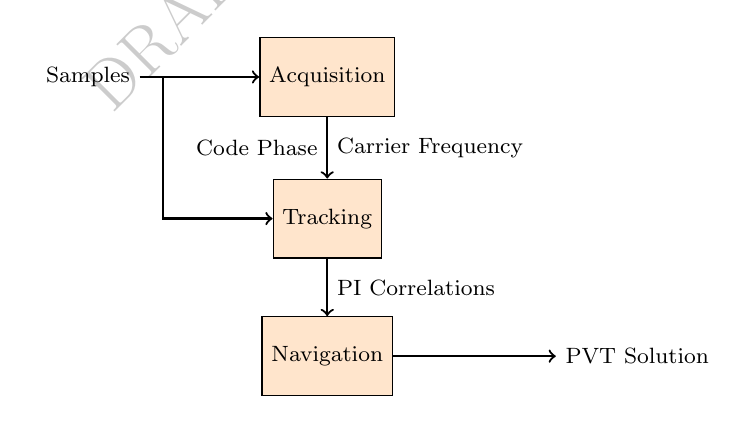
\begin{tikzpicture}

  \tikzstyle{block} = [draw, fill=orange!20, rectangle, minimum height=1.0cm, line width=0.5pt]

  \matrix (foo) [matrix of nodes, column sep=0.3cm,row sep=0.15cm, anchor=center, 
                 nodes={anchor=center,font=\footnotesize}]
  {
    \node[left] (samples) {Samples}; & \node[coordinate] (input) {}; & \node[block] (acq) {Acquisition}; &  \\ %First Row
     & & \node[left] {Code Phase}; \node[right] {Carrier Frequency}; &  \\ %Second Row
     & & \node[block] (track) {Tracking}; & \\ %Third Row
     & & \node[left] {}; \node[right] {PI Correlations}; &  \\ %Fourth Row
     & & \node[block] (nav) {Navigation}; & \node[right] (output) {PVT Solution}; \\ %Fifth row
  };

  \draw[-,color=black!100,thick] (samples) -- (input);
  \draw[->,color=black!100,thick] (input) -- (acq);
  \draw[->,color=black!100,thick] (input) |- (track);
  \draw[->,color=black!100,thick] (acq) -- (track);
  \draw[->,color=black!100,thick] (track) -- (nav);
  \draw[->,color=black!100,thick] (nav) -- (output);
  
\end{tikzpicture}
\captionof{figure}[ToC entry]{Typical GPS Receiver Signal Flow}
\end{center}

The acquisition and tracking blocks perform essentially the same DSP operation - a correlation of
the incoming baseband samples with a locally generated carrier and spreading code, as represented
by the below equation:
\normalfont\small
\begin{center}$y_{out}=\displaystyle\sum\limits_{n=0}^{N-1}x_{in}(n)e^{j\omega_{c} nt_s}c_{s}(n)$ ,
where
\end{center}
$y_{out}$ : resultant correlation (complex)\\
$N$ : correlation length \\
$x_{in}$ : incoming samples \\
$e^{j\omega_{c} nt_s}$ : local carrier (complex)\\
$\omega_{c}$ : local carrier frequency in radians \\
$t_{s}$ : sampling period \\
$c_s$ : spreading code \\

\normalfont\normalsize

This operation requires 2 multiplications and an addition for both the real and imaginary parts
of the correlation, or 2 multiplications and 2 multiply-accumulates (MACCs). In order to track the
spreading code, we typically use half-chip spaced early, prompt, and late code correlations, which
brings this total to 6 multiplications and 6 MACCs per tracking correlator. If we assume a sampling
frequency of 16.368MHz (as in the Swift Navigation system), 8 tracking correlators, and a continuously 
running acquisition correlator, then we have approximately $800*10^6$ multiplications and MACCs per 
second. FPGA's are well suited to this sort of repetitive, parallelized number crunching, and hence
the choice for our system architeture.

\pagebreak

\section{Clock}

All of the SwiftNAP's clocking resources are driven by the 16.368MHz CLKOUT pin of the MAX2769 Frontend.
The table below shows how each peripheral in the SwiftNAP is clocked relative to the 16.368MHz input.
\begin{center}
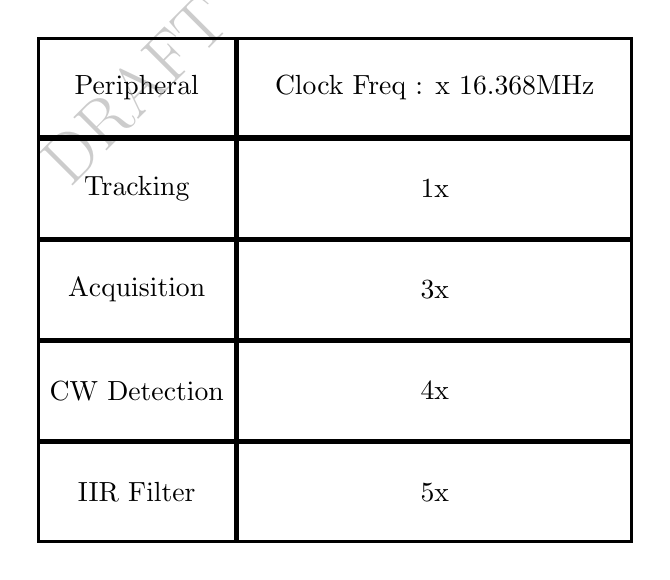
\begin{tikzpicture}
  \tikzstyle{fc}=[
    draw, rectangle, thick,
    minimum height=2.5cm,
    minimum width=5cm,
    line width=1.0pt,
    font=\huge,
    scale=0.5
  ]
  \tikzstyle{sc}=[fc,
    minimum width = 10cm
  ]

  \matrix [matrix of nodes]
  {
    |[fc] (peripheral) {};| & |[sc] (clock frequency) {};| \\
    |[fc] (track) {};|      & |[sc] (track freq) {};| \\
    |[fc] (acq) {};|        & |[sc] (acq freq) {};| \\
    |[fc] (cw) {};|         & |[sc] (cw freq) {};| \\
    |[fc] (iir) {};|        & |[sc] (iir freq) {};| \\
  };

  \node[] at (peripheral) {Peripheral}; \node[] at (clock frequency) {Clock Freq : x 16.368MHz}; 
  \node[] at (track) {Tracking};        \node[] at (track freq) {1x}; 
  \node[] at (acq) {Acquisition};       \node[] at (acq freq) {3x}; 
  \node[] at (cw) {CW Detection};       \node[] at (cw freq) {4x}; 
  \node[] at (iir) {IIR Filter};        \node[] at (iir freq) {5x}; 
  
\end{tikzpicture}
\end{center}

\subsection{Frontend clock frequency}
\subsection{SPI clock frequency}

\section{Communication Interface}
\subsection{SPI}
\subsection{Timing Strobe}
\subsection{Interrupt Line}
\subsection{Pipelining}

\section{Loadable Code RAM}
\subsection{Loading sample RAM}

\section{Sample RAM}
\subsection{Loading code RAM}

\section{Interrupt Request Register}

\section{Error Register}

\section{Register Addresses}

\section{Acquisition Channel}
\subsection{Overview}
\subsection{Registers}
\subsubsection{Load}
\subsubsection{Init}
\subsubsection{Corr}
\subsection{How to use acquisition channel}
\subsubsection{Loading sample RAM}
\subsubsection{Loading code RAM}
\subsubsection{Starting acquisition}
\subsubsection{Servicing interrupts}
\subsubsection{Stopping acquisition}

\section{Tracking Channel}
\subsection{Overview}
\subsection{Registers}
\subsubsection{Load}
\subsubsection{Init}
\subsubsection{Update}
\subsubsection{Corr}
\subsubsection{Phase}
\subsection{How to use tracking channel}
\subsubsection{Loading code RAM}
\subsubsection{Starting tracking}
\subsubsection{Servicing interrupts}
\subsubsection{Stopping tracking}

\section{CW Detection Channel}
\subsection{Overview}
\subsection{Registers}
\subsubsection{Load}
\subsubsection{Init}
\subsubsection{Corr}
\subsection{How to use CW Detection channel}
\subsubsection{Loading sample RAM}
\subsubsection{Starting CW Detection}
\subsubsection{Servicing interrupts}
\subsubsection{Stopping CW Detection}

\section{IIR Filter}
\subsection{Overview}
\subsection{Registers}
\subsubsection{Coefficients}

\section{Foobar}
\large
\label{sec:Features}
\begin{itemize}
  \bulletnoindent
  \item Item 1.
  \item Item 2.
  \item Item 3.
\end{itemize}
\normalsize

\titleformat*{\section}{\color{alt}\normalfont\huge\bfseries}

\subsection{Skrillex}

\end{multicols} 

\end{document} 
